%============================================================================
% tento soubor pouzijte jako zaklad
% (c) 2008 Michal Bidlo
% E-mail: bidlom AT fit vutbr cz
%============================================================================
% kodovaní: utf8 (zmena prikazem iconv, recode nebo cstocs)
%----------------------------------------------------------------------------
% zpracování: make, make pdf, make desky, make clean
% připomínky posílejte na e-mail: bidlom AT fit.vutbr.cz
% vim: set syntax=tex
%============================================================================
\documentclass[english]{jtulak} % odevzdani do wisu - odkazy, na ktere se da klikat
%\documentclass[cover,print]{fitthesis} % pro tisk - na odkazy se neda klikat
%\documentclass[english,print]{fitthesis} % pro tisk - na odkazy se neda klikat
%      \documentclass[english]{fitthesis}
% * Je-li prace psana v anglickem jazyce, je zapotrebi u tridy pouzit 
%   parametr english nasledovne:
%      \documentclass[english]{fitthesis}
% * Neprejete-li si vysazet na prvni strane dokumentu desky, zruste 
%   parametr cover

% zde zvolime kodovani, ve kterem je napsan text prace
% "latin2" pro iso8859-2 nebo "cp1250" pro windows-1250, "utf8" pro "utf-8"
%\usepackage{ucs}
\usepackage[utf8]{inputenc}
%\usepackage[T1, IL2]{fontenc}
\usepackage{url}
\DeclareUrlCommand\url{\def\UrlLeft{<}\def\UrlRight{>} \urlstyle{tt}}

%zde muzeme vlozit vlastni balicky

\usepackage{sidecap}
\usepackage{listings}
\usepackage{syntonly}
%\syntaxonly

% =======================================================================
% balíček "hyperref" vytváří klikací odkazy v pdf, pokud tedy použijeme pdflatex
% problém je, že balíček hyperref musí být uveden jako poslední, takže nemůže
% být v šabloně

\ifx\pdfoutput\undefined % nejedeme pod pdflatexem
	\usepackage[dvips]{color, graphicx}
	\usepackage[tex4ht]{hyperref}
\else
  \ifNotPrint
    \usepackage{color}
    \usepackage[unicode,colorlinks,hyperindex,plainpages=false,pdftex]{hyperref}
    \definecolor{links}{rgb}{0.4,0.5,0}
    \definecolor{anchors}{rgb}{1,0,0}
    \hypersetup{
      colorlinks,
      citecolor=Green,
      %linkcolor=links,
      %urlcolor=links
      }
    \def\AnchorColor{anchors}
    \def\LinkColor{links}
    \def\pdfBorderAttrs{/Border [0 0 0] }  % bez okrajů kolem odkazů
    \pdfcompresslevel=9
  \fi
\fi

%Informace o praci/projektu
%---------------------------------------------------------------------------
\projectinfo{
  %Prace
  project=BP,            %typ prace BP/SP/DP/DR
  year=2014,             %rok
  date=\today,           %datum odevzdani
  %Nazev prace
  title.cs={RdRand: IA-64 a IA-32 instrukce pro generování náhodných čísel},  %nazev prace v cestine
  title.en={RdRand: IA-64 and IA-32 Instruction for Random Number Generation}, %nazev prace v anglictine
  %Autor
  author={Jan Ťulák},   %jmeno prijmeni autora
  %author.title.p=Bc., %titul pred jmenem (nepovinne)
  %author.title.a=PhD, %titul za jmenem (nepovinne)
  %Ustav
  department=UPSY, % doplnte prislusnou zkratku: UPSY/UIFS/UITS/UPGM
  %Skolitel
  supervisor= Tomáš Kašpárek, %jmeno prijmeni skolitele
  supervisor.title.p=Ing.,   %titul pred jmenem (nepovinne)
  supervisor.title.a={},    %titul za jmenem (nepovinne)
  %Klicova slova, abstrakty, prohlaseni a podekovani je mozne definovat 
  %bud pomoci nasledujicich parametru nebo pomoci vyhrazenych maker (viz dale)
  %===========================================================================
  %Klicova slova
  keywords.cs={RdRand, Entropie, Ivy Bridge, IA-32, IA-64, náhodná čísla}, %klicova slova v ceskem jazyce
  keywords.en={RdRand, Entropy, Ivy Bridge, IA-32, IA-64, random numbers}, %klicova slova v anglickem jazyce
  %Abstract
  % abstrakt v ceskem jazyce
  abstract.cs={Tato práce popisuje implementaci a testování Linuxové knihovny,
  vytvořené pro poskytnutí abstrakce mezi uživatelem a instrukcí RdRand 
  od Intelu (Ivy Bridge RNG). Samotná instrukce je rovněž zběžně popsána a jsou ověřeny některé její vlastnosti, jako kryptografická bezpečnost výstupních dat a reálná rychlost této instrukce.},
  % abstrakt v anglickem jazyce
  abstract.en={This thesis describes implementation and testing of a~Linux 
  library, created for providing an~abstraction layer between a~user and 
  the~Intel's RdRand instruction (Ivy Bridge RNG). The~instruction itself is briefly described and some of its properties are tested
  here, like cryptographic strength of its output and the real speed of the instruction.}, 
  %Prohlaseni
  declaration={Hereby I declare that I wrote this work on my own and all used sources are stated and correctly noted as citations.},
  %Podekovani (nepovinne)
  acknowledgment={I want to thank to Jiří Hladký, my supervisor in Red Hat for all his help and ideas.}, % nepovinne
  % Rozsireny abstrakt v ceskem jazyce
  abstractext.cs={Počínaje generací Ivy Bridge, Intel začal vybavovat své procesory hardwarovým generátorem náhodných čísel. Tento generátor, pojmenovaný Intel Secure Key, je možné využívat pomocí strojové instrukce RdRand pro rychlé získání náhodných čísel s vysokou entropií.\\
 \\
 Intel Secure Key je založen na tepelném šumu ovlivňujícím chování dvou vzájemně propojených invertorů. Tyto invertory jsou oba nejprve nastaveny do stejného stavu 1 (tedy jsou nestabilní) a po následném odpojení řídící části se jeden z nich přepne do stavu 0. Pravděpodobnost překlopení konkrétního invertoru by měla být 1:1 a podle toho, který invertor se překlopil, je vygenerován jeden bit. Na tento jednoduchý generátor navazuje filtrovací logika, která se snaží odstranit korelace mezi vygenerovanými hodnotami. Protože tato logika výrazně zpomaluje generování, je její výstup použit jako neustále se měnící inicializační vektor pseudonáhodného generátoru založeného na AES algoritmech.\\
 \\
Rychlost RdRandu by podle Intelu měla dosahovat až 800 MiB/s, přičemž rychlost dostupná pro jednu výpočetní jednotku procesoru odpovídá 800 / počet jednotek. Reálné zkušenosti s RdRandem jsou však malé a jeho využití není zatím příliš rozšířeno. Bylo tedy nutné provést výkonnostní testy a ověřit jak tato tvrzení, tak statistické vlastnosti generátoru. \\
\\
Statistické testy výstupu generátoru nenalezly žádné chyby ani v několika desítkách TB dat. Výkonnostní testy potvrdily, že rychlost RdRand instrukce na procesorech generace Ivy Bridge se blíží udávané rychlosti a pro její dosažení je třeba využít všech výpočetních jednotek. V následující generaci je však výkon pouze poloviční, zřejmě kvůli změnám v architektuře. Tato informace byla následně potvrzena Intelem.\\
\\
S ohledem na odhalení aktivit NSA Edwardem Snowdenem ve věci úmyslného oslabování kryptografických standardů a spolupráce s výrobci  HW a SW je vhodné věnovat zvýšenou pozornost i bezpečnosti tohoto generátoru náhodných čísel. V textu práce jsou zběžně popsány některé možnosti, jak by RdRand mohl negativně ovlivnit bezpečnost systému, který jej využívá. Z možných vektorů útoku lze jmenovat například změnu elektrických vlastností polovodiče vedoucí k odlišnému chování, která přitom není zjistitelná ani při optické inspekci čipu.\\
\\
K RdRandu je možné přistupovat i skrz API poskytované knihovnami jako je OpenSSL. To je však komplikovanější, než v případě úzce zaměřené knihovny. Jednak to přináší řadu závislostí na dalších knihovnách a jejich verzích a jednak je takové rozhraní zbytečně komplikované.\\
\\
Část software vytvořeného pro tuto práci byla tedy uvolněna jako knihovna pro operační systém Linux, poskytující abstrakci nad instrukcí RdRand a umožňující snadno generovat větší množství dat, než 16/32/64 bitů poskytovaných instrukční sadou procesoru. Rovněž testování, zda konkrétní procesor disponuje touto instrukcí bylo zjednodušeno, neboť AMD pracuje na vlastní variantě generátoru náhodných čísel na procesoru a tato knihovna může být snadno rozšířena i pro další implementaci. Vytvořená knihovna má jen minimální závislosti na dalším SW.},
}

%Abstrakt (cesky, anglicky)
%\abstract[cs]{Do tohoto odstavce bude zapsán výtah (abstrakt) práce v českém jazyce.}
%\abstract[en]{Do tohoto odstavce bude zapsán výtah (abstrakt) práce v anglickém jazyce.}

%Klicova slova (cesky, anglicky)
%\keywords[cs]{Sem budou zapsána jednotlivá klíčová slova v českém jazyce, oddělená čárkami.}
%\keywords[en]{Sem budou zapsána jednotlivá klíčová slova v anglickém jazyce, oddělená čárkami.}

%Prohlaseni
%\declaration{Prohlašuji, že jsem tuto bakalářskou práci vypracoval samostatně pod vedením pana X...
%Další informace mi poskytli...
%Uvedl jsem všechny literární prameny a publikace, ze kterých jsem čerpal.}

%Podekovani (nepovinne)
%\acknowledgment{V této sekci je možno uvést poděkování vedoucímu práce a těm, kteří poskytli odbornou pomoc
%(externí zadavatel, konzultant, apod.).}

%%%%%%%%%%%%%%%%%%%%%%%%%

% my macro for function declaration
\newcommand{\FunctionDeclareNE}[4]{%
  \noindent
  \ifdefined\hyperref
    \phantomsection
  \fi
  \label{fnt:#2}
  \textbf{{\em #1} {\tt #2} ( {\em #3} ) }-- {#4}
  \endgroup}
% because underscore is a special character and has to be escaped
% but escaped sequences must not be in \label
\def\FunctionDeclare{\begingroup 
\catcode`\_=12
\FunctionDeclareNE}

% my macro for linking to a function declaration
\newcommand{\functionNE}[1]{%
  \ifdefined\hyperref
    \hyperref[fnt:#1]{\tt #1}%
  \else
    {\tt #1}%
  \fi
\endgroup}
% because underscore is a special character and has to be escaped
% but escaped sequences must not be in \label
\def\function{\begingroup 
\catcode`\_=12
\functionNE}

%%%%%%%%%%%%%%%%%%%%%
% my macro for function declaration
\newcommand{\MachineDeclareNE}[4]{%
  \noindent
  \ifdefined\hyperref
    \phantomsection
  \fi
  \label{machines:#1}
  \textbf{#1}\\
    CPU: {\it #2}\\
    RAM: {\it #3}\\
    Notes: {\it #4}\\
  \endgroup}
% because underscore is a special character and has to be escaped
% but escaped sequences must not be in \label
\def\machineDeclare{\begingroup 
\catcode`\_=12
\MachineDeclareNE}

\newcommand{\machineNE}[1]{%
  \ifdefined\hyperref
    \hyperref[machines:#1]{\it #1}%
  \else
    {\it #1}%
  \fi
\endgroup}
% because underscore is a special character and has to be escaped
% but escaped sequences must not be in \label
\def\machine{\begingroup 
\catcode`\_=12
\machineNE}


%%%%%%%%%%%%%%%%%%%%%

\begin{document}

\pagenumbering{Alph}
  % Vysazeni titulnich stran
  % ----------------------------------------------
  \maketitle
  
  % Obsah
  % ----------------------------------------------
\pagenumbering{arabic}
  \tableofcontents
  
  % Seznam obrazku a tabulek (pokud prace obsahuje velke mnozstvi obrazku, tak se to hodi)
  % \listoffigures
  % \listoftables 

  % Text prace
  % ----------------------------------------------
  %=========================================================================
% (c) Jan Tulak (2013)

%=========================================================================
\chapter{Introduction}
\TODO{Slovosled!} %TODO slovosled!
Generating of~true random numbers is a~stochastic process. In opposite, computers are deterministic machines and as such, they are unable to~generate true random numbers just using abilities of~a~Turing machine. \TODO{quote it} %TODO quote it
But random numbers are crucial in cryptography and once computers began to be used in this domain, \TODO{more details} %TODO more details
people tried combine these two conflicting requests - to~allow a~deterministic machine to act stochasticaly. 

There are two solutions of~this problem. We can stay with completely deterministic machines and through series of~mathematical operations compute pseudo random numbers, that seems to be random, but when using the~same initial state and algorithm, we get the~same numbers again. Or we can add some source of~entropy to the~system, a~device that is physically stochastic and measure its output (wherever it be temperature, radiation, or anything else what can be later, directly or indirectly, converted to electric current). The second approach is providing real random numbers, but frequently with much lower speed, than pseudo-random algorithms. Also, finding an entropy source with a~good speed, an~uniform distribution and with a~reliable price, size, energy consumption and other parameters is difficult, so frequently the~generated random values are used as a~seed for a~pseudo-random algorithm, which can lead to great speed enhancement without loosing much of~the~randomness.

The problematic of~quality of~the~entropy for a~specific purpose is wide and this work is not intended to cover it to great length, but still it has be shortly mentioned. Clearly, different requests has an developer of~a~video game, a~researcher performing a~simulation and an~army for encrypting their information. The researcher needs numbers that seems to be random, but aren't - he or she needs to be able to repeat the~simulation with the~same initial state to get the~same result\footnote{In some cases of~computing, researchers are even keeping the~same machines, as a~different machine would provide a~different results due to inner number representation and architecture differences.\cite{ArithmeticInCloud}\TODO{Is it ok?}%TODO is it ok?
}
The video game developer can also need the~repeatibility (e.g. for generating a~terrain), but in another case, like decisions of~a~artificial intelligence, the~repeatibility may not be requested and in case of~gambling highly unwanted. And the~army needs the~random numbers generator to be completely stochastic to prevent an enemy to decipher their messages. Each of~these cases has different requests for quality, speed and price.

Due to prices of~{\em Hardware Random Number Generators (HW RNG)}, they were for long time domain of~just governments and big corporations,\TODO{Quote it}%TODO quote it - security oriented CPUs with HW RNGs...
leaving the~consumer electronic to rely only on {\em Pseudo-Random Number Generators (PRNG)}. PRNG algorithms developed to great success over time, providing enough entropy for usual needs of~ordinary people and also for most of~cryptographic needs ({\em Cryptographically Secure Random Number Generators - CSPRNG}), but still it needs to be seeded by data with at least some entropy from the~beginning. And as more and more of~our daily life depends on computers, the~importance of~keeping our data secured raised up. 

In 2012\cite{IntelRdRandFindAbout} Intel added a~Digital Random Number Generator (DRNG) on their chips and allowed programmers to use it as part of~instruction set of~that CPUs. Intel named the~instruction RdRand and its own implementation and the~underlying DRNG hardware implementation is named {\em Intel Secure Key} (previously code-named Bull Mountain Technology)\cite{IntelDRNGAnalysis}. Intel used combination of~HW RNG and CSPRNG, solution known as {\em Cascade Construction RNG}, where the~relatively slow HW RNG works as a~seed generator for much faster CSPRNG. As is showed later in this thesis, in \fullref{sec:performance-testing}, the~difference in speed is about thousand times.

This step brought HW RNGs to general public, but the~limitation on just Intel CPUs means that there is still big part of~the~information technology market without such solution - in x86 world there is also AMD who did not yet implemented this instruction and also many of~different architectures, like ARM, in mobile devices. So the~programmers cannot count on the~presence of~a~HW RNG on a~casual computers yet. Furthermore, the~Intel's RdRand instruction is still mostly unknown and there are also a~questions about reliability of~this generator, which is sealed into the~chip and unable to be audited\cite{TheodoreTsoNSA} if it is really manufactured according of~published scheme\cite{AnalysisOfDRNG} or if there is not a~backdoor. There is important to notice that if there could be a~backdoor in the~RNG, there could be backdoors also in any other part of~the~CPU, opening possibilities for many others attacks which could achieve the~same result.

As I'm interested in computer security on some level, as well as in Linux, when I got the~possibility to work on implementation of~a~library using RdRand, as well as test it, in production environment of~Red Hat corporation, I was interested in it and choose it as my thesis. During the~work, we have discovered unexpected issue with performance on some CPUs which was handed to Intel, yet until now without a~response.

Because now, in 2013, no other implementation of~RdRand than Intel's one exists\footnote{Although AMD is working on their own implementation.\TODO{Find more about it }},%TODO find more about it - http://extrahardware.cnews.cz/cpu-architektury-excavator-budou-umet-avx2-rdrand-dalsi-nove-instrukce
the term {\em RdRand} is used just as the~instruction implemented by {\em Intel Secure Key} technology.

\TODO{Update it when news come.}%TODO Update it when news come.


%========================================================================= 


%========================================================================= 
\chapter{Random Numbers And Deterministic Machines}\label{chap:randomNumbers}

The term {\em Entropy} is usually used  as the {\em measure of disorder and uncertainty of a system}.\cite{Entrophy}. Claude E. Shannon defined it for information theory as the average of uncertainty (unpredictability) of an information source~\cite[p.~396]{AMathematicalTheoryOfCommunication}. The important properties of an information source with high entropy are~\cite[p.~150]{CryptographyAndNetworkSecurity}: 
\begin{description}
 \item [Uniform distribution:] Probability of each value should be the same, no values should be generated with higher frequency of occurrence than others.
 \item [Independence:] No one value can be inferred from the others.
\end{description}


In this report the term {\em entropy} can also refer to a random value itself from an information source. 



\section{Pseudorandom Numbers}
When we pass any value to a {\em pseudorandom number generator} (PRNG), the PRNG will produce a long sequence of values, that seems to be random and statistical tests on these sequences (if the PRNG is strong enough) should not find any correlation between the produced values. However, the produced sequence is finite and thus after a time it become to repeat itself. This is because the PRNG is just an implementation of an algorithm, computing mathematical operations on the previously computed value (on the start of the PRNG, we need to fill it with a {\em seed} - a starting value) and after finite count of steps the algorithm gets to the point of its start.

A simple example of such PRNG, one of the most basic but the most widely used~\cite[p.~151]{CryptographyAndNetworkSecurity}, is the {\em linear congruential random number generator} (LCRNG) defined as 
\begin{equation}\label{eq:LCRNG}
  X_n = (aX_{n-1} + b) \mod{m}
\end{equation}
where $X_n$ is the $n$th number of the sequence ($X_{n-1}$ respectively the previous). $a$, $b$ and $m$ are constants and the selected values has big impact on quality of the output. $X_0$ is a seed. 

The LCRNGs are still useful because of their speed and easy implementation in various noncryptographic situations, when their disadvantages (most importantly their predictability~\cite[p.~152, 153]{CryptographyAndNetworkSecurity}) are not important.~\cite[chapter~16.1]{AppliedCryptography}. 

Because with knowing the initial seed we can repeat all the pseudorandom sequence, it is important to have a secure, random seed if we want to use a PRNG in cryptography, except of having a {\em cryptographicaly secure pseudorandom number generator} (CSPRNG). In computers, the seed can be frequently extracted from hard-to-predict events like user interaction or network communication.

We can say a sequence generator is pseudorandom, if its output looks random, even under statistical tests.

\subsection{Cryptographically Secure PRNG}
Encryption algorithms can be sometimes used as the PRNG, for example DES or AES. These provides a very good results~\cite[p.~153-156]{CryptographyAndNetworkSecurity}.

The important property of a PRNG, that can be considered as cryptographically secure, is {\em unpredictability}. That means that it is impossible under our computational knowledge to predict (forward or backward) any number, even if we know the used algorithm\footnote{This is the reason, why LCRNGs are not considered as CSPRNGs - if an attacker have just 3 following numbers of the basic LCRNG, $X_{i}$, $X_{i+1}$ and $X_{i+2}$, he can create an equation for each of them from the equation~\ref{eq:LCRNG} $X_n = (aX_{n-1} + b)$~mod~$m$. The three equations creates a system of equations with 3 unknowns $a$, $b$ and $m$, which is very easy to solve. After solving it, the attacker knows all the constants and then he can compute any preceding or following number in the sequence.} and/or the entropy source(s). The forward/backward security has to apply also for cases when the inner state of the RNG is disclosed, for example by reading it in memory.

The {\em forward security} grant us, that knowing of the current state of the generator, it is not possible to learn the previously generated values. The {\em backward security}, also known as {\em break-in recovery}  means, that even if an attacker knows the state of the generator in a specific time, it is not possible recover the state and thus predict future values.

\section{True Random Numbers}
To produce random values, {\em true random number generators} (TRNGs), are using physical events that are hard to be predicted. The TRNGs can measure absolute values, timing or occurrence of such events.
An examples of what can be used for generating true random numbers are radioactive decay, avalanche effects on reverse-biased electronic components and thermal, atmospheric and other sources of noise, and others~\cite[p.~6]{AnalysisOfEntropyLevels}.

However, real using of such devices is problematic. The sources of entropy are frequently somehow biased and cyclic, so it is necessary to have an online testing and filtering, which is usually significantly slowing the output speed. Also, the price can be a problem too\footnote{From hundreds to thousands of Euro. For a brief overlook, see a comparison on Wikipedia~\cite{HWRNGComparison}. \TODO{Is is usage of wiki all right?}}.


\section{Random Numbers In Linux}\label{sec:randomNumbers:linux}
The {\em Linux random number generator} (LRNG) is gathering its entropy from events that are very hard to predict: mouse movements, key-presses, interrupt sources of the system, jitter of access times to disks. These events are saved with a timestamp into an entropy pool~\cite{AnalysisOfLinuxRNG}.

LRNG is offering an API for its use. Except of C function {\tt get\_random\_bytes}, it also provides two device drivers, {\tt /dev/random} and {\tt /dev/urandom}. The difference between these two devices is in way, how they handle user requests, providing two different levels of security. The {\tt /dev/random} is producing more secure randomness and if there is not enough entropy in the entropy pool, then it can block the reader, until enough entropy is gathered. {\tt /dev/urandom} then never blocks its output and produce less secure values, but is faster\footnote{Just for illustration, the speed of {\tt /dev/random} on my machine is about 300-400 kiB/s, while {\tt /dev/urandom} is about 16 MiB/s}~\cite[chapter~1]{AnalysisOfLinuxRNG}. 

The LRNG is composed from three independent, asynchronous processes. Firstly, there is the collection of the entropy from all system. In the second process, the entropy is saved into the entropy pool and on last, when a random value is requested, the third process generates it using SHA-1 algorithm\footnote{In all the process, the only one non-linear cryptographic function is SHA-1, that is used three times, along with some register shifting and pool mixing~\cite[section~2.6]{AnalysisOfLinuxRNG}.}~\cite[chapter~2]{AnalysisOfLinuxRNG}.

\begin{figure}[h!]
  \centering
 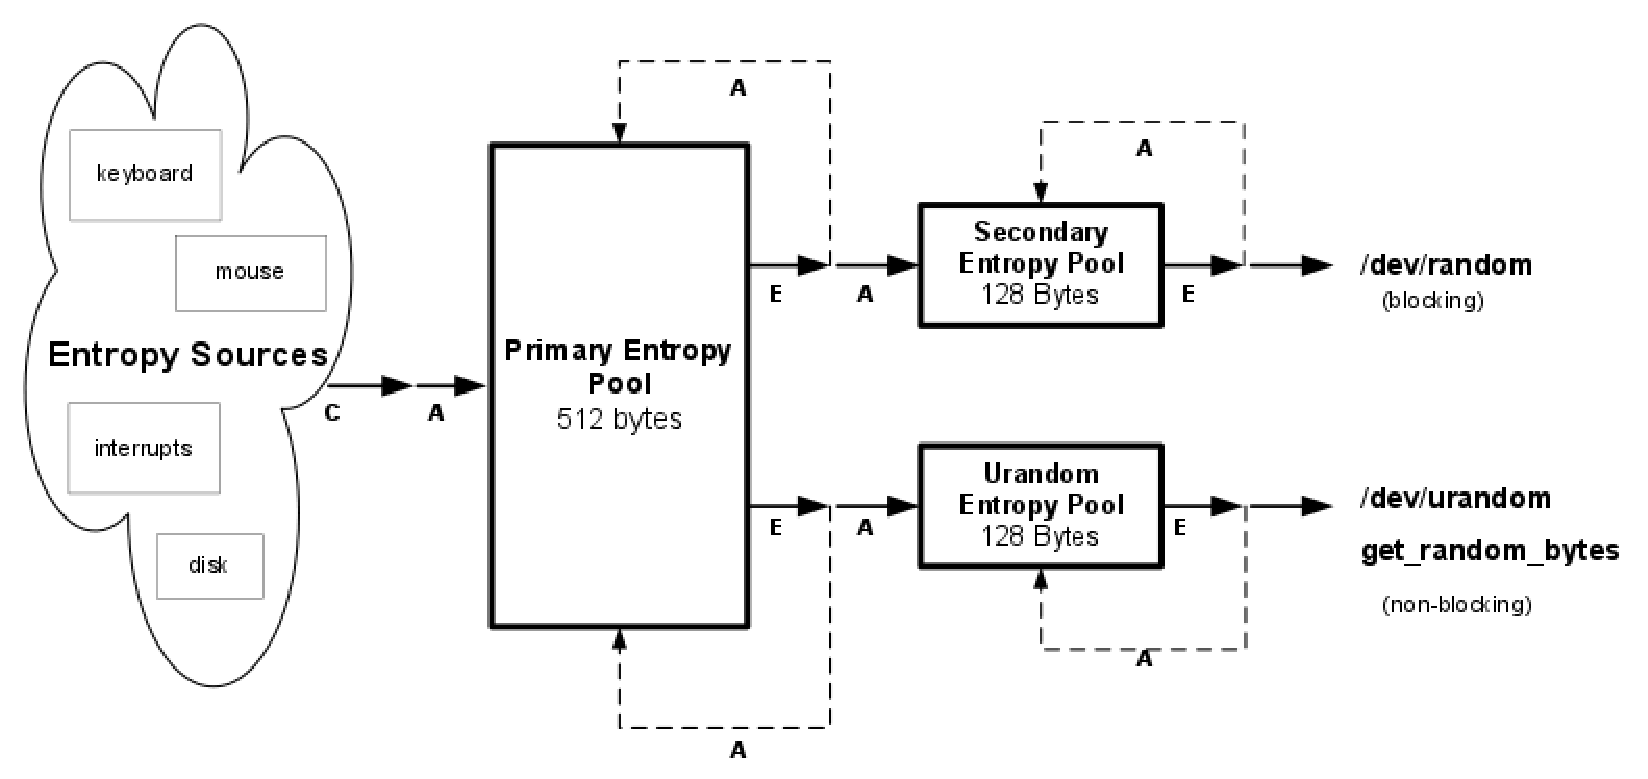
\includegraphics[width=16cm,keepaspectratio]{fig/LRNG} % Or .pdf
%\includegraphics[width=10cm,keepaspectratio]{fig/ISK-scheme}
\caption{Scheme of the LRNG. The entropy is collected (C) and added (A) to the primary pool. Entropy is extracted (E) from the secondary or urandom pool. Whenever entropy is extracted from a pool, some of it is also fed back into this pool (broken line). The secondary pool and the urandom pool draw entropy from the primary pool~\cite{AnalysisOfLinuxRNG}.}
\label{fig:LRNG}
\end{figure}

When a random value is generated, the process uses the relevant secondary or urandom pool as the seed and the level of entropy in the pool is lowered. When the level of entropy is too low, the pool is refreshed from the primary pool. In case of low entropy in all pools, the blocking {\tt /dev/random} waits until the system gathers more entropy, while {\tt /dev/urandom} just generates randomness from any entropy it has.

%-------------------------------------------------------------------------


\section{Summary}
As was noted, good true random number generators are hard to find, especially for an end-user usage. Although physical computers has some sources of entropy, with moving to virtualized systems the sources are disappearing~\cite{AnalysisOfEntropyLevels} and furthermore, with raising requirements of security, the importance of good random numbers is more important than before.

Also, as is showed in {\em Analysis of the linux random number generator}~\cite{AnalysisOfLinuxRNG}, even kernel generators can has security flaws and allow some form of forward or backward attack. 

For these reasons, it would be useful to have widely accessible and widespread fast and high quality TRNG or at least slower TRNG with CSPRNG. That device should be available to all users, even within virtualized systems. How RdRand can help with these points is shown in other chapters of this thesis.


%============================================================
\chapter{The RdRand instruction}  \label{chap:rdrand-instruction}
\par{
First public information about RdRand came sometime during year 
2011\cite{IntelRdRandFindAbout}, a~year before the~CPUs with it were released
 and Intel itself send patches to add support into Linux in summer of~the~same 
 year\cite{KernelRdRand}. Later, RdRand was added between Linux entropy 
 sources for {\tt /dev/[u]random}. According to known 
 information~\cite{TheodoreTsoNSA}, Intel tried to have {\tt /dev/[u]random} rely
  only on their instruction, but that was denied. 
}

\par{
After disclosure of~extends of~NSA spying activities by Edward Snowden 
in summer of~2013\cite{GuardianNSA,DailymailNSA}, a~petition for removing 
RdRand from Linux entropy sources was created~\cite{PetitionRdRand}. 
Although supported by just 8 signatures, it got wide attention on 
information-technology aimed news pages and magazines, like Slashdot.org~\cite{PetitionRdRandSlashdot}. The petition was closed after Linus Torvalds 
responds with scorn:
}
\begin{quote} \par{\dots}
\par{
Short answer: we actually know what we are doing. You don't.
}
\par{
Long answer: we use rdrand as \_one\_ of~many inputs into the~random pool, 
and we use it as a~way to \_improve\_ that random pool. 
So even if rdrand were to be back-doored by the~NSA, our use of~rdrand 
actually improves the~quality of~the~random numbers you get 
from {\tt /dev/random}.
}
\par{\dots}
\end{quote}

\section{History}\label{sec:intel-history}
\par{
This is not for the first time Intel is producing a HW RNG. Around 1999, 
their chipsets of 8xx series had a TRNG~\cite{Intel810Manual}[chapter 1.3.5]\cite{RNGTools} 
as part of the Intel FWH (82802AB or 82802AC) component.
This RNG was analog -- a thermal noise was affecting a resistor. 
The noise was amplified and forwarded to a voltage--controlled oscillator. 
Its output was combined with another oscillator with much higher frequency 
and the drift between these two frequencies provided the requested entropy~\cite{IntelRNGAnalysis}.
}
\par{
Pairs of generated bits were digitally processed, using Von Neumann Corrector to enhance its statistical properties by removing some bias. Due to this, the RNG has a variable bitrate, averaging around 75 Kbit/sec.
}
\begin{table}[h!]
  \begin{center}
    \begin{tabular}{|c|c|}
      \hline
      Input Bits &  Output\\
      \hline  
      0, 0 & None\\
      0, 1 & 1\\
      1, 0 & 0\\
      1, 1 & None\\
      \hline
    \end{tabular}    \caption{A Von Neumann corrector}
    \label{fig:VonNeumannCorrector}
  \end{center}
\end{table}
% --------------------------------------------------------
\section{Intel Secure Key}\label{sec:intel-secure-key}
\par{
The Intel Secure Key (ISK) uses cascade construction, combining a~HW RNG
 with CSPRNG into one sealed block on CPU, which is compliant with many 
 security standards, including NIST SP800-90, FIPS-140-2, and ANSI 
X9.82\cite{IntelDRNGGuide}. Although it is impossible to audit it, there was found 
 no evidence of~low entropy or anything that would deny the~security standards 
 compliance - neither with tests in \fullref{sec:testing:stat-testing}, nor any other 
 tests anyone else did\footnote{I assume that such revelation would become 
 quickly known and broadly discussed, but all tests I have found have 
 the same conclusion as mine.}.
 }

% --------------------------------------------------------
\section{Physical Implementation}\label{sec:ISK-physical}
\par{
One important thing about ISK with a big impact on the performance, but also price 
of~that solution is that there is only one unit on a~die and the~unit should be
 the~same on all CPUs\footnote{We didn't find the "be the same" officially confirmed and it can change in future CPUs. But empirical test results made on range of different CPU types provided the same characteristics, with exception of Intel Xeon CPUs as is described in the \ref{chap:testing}.}.~\cite{IntelDRNGGuide}[Chapter 3.1]
Because all processing units (PUs)\footnote{Two physical cores with 
hyper-threading counts as four PUs.} on one die share the~RNG, one thread 
reading random numbers from it can never be faster than 
$Total speed  \frac{1}{PUs}$. The effect of~this is that the~performance is
 scalable until amount of PUs and the maximum output speed are exceeded 
 (see \fullref{sec:testing:performance-testing}), and price of~the~CPU is less 
 affected.
}

\par{
Each ISK unit consists three basic parts: A hardware entropy source, 
a~conditioner and a~{\em deterministic random bit generator} (DRBG)
\cite{IntelDRNGGuide}. The frequency of~the~RNG is independent 
on the~rest of~the~CPU and is set to 800 MHz. 
}
\begin{figure}[h!]
  \centering
 \includegraphics[width = 10cm,keepaspectratio]{fig/ISK-scheme.pdf} % Or .pdf
%\includegraphics[width=10cm,keepaspectratio]{fig/ISK-scheme}
\caption{An Intel Secure Key unit}
\label{fig:ISK-unit}
\end{figure}


% ....................................................
\subsection{Entropy Source}
\par{
The entropy source is a~metastable circuit, with unpredictable behavior based 
on thermal noise.~\cite{UnderstandingRdRandElectronic}
In figure~\ref{fig:ES-circuit}, the~middle (red) part is the~heart 
of~the~circuit, a~RS-NOR latch. As its {\em reset} and {\em set} inputs 
are wired together, when an impulse is brought on these inputs, the~latch sets 
to 1 or 0 based on thermal noise. To provide better distribution, there is 
the~bottom (blue) negative feedback. Based on the~output of~the~latch, charge 
on capacitors in the~negative feedback is adjusted and then this negative 
feedback slightly shift the~chance for next bit to be opposite. The longer 
is a~sequence of~the~same bits, the~higher charge is on the~capacitors 
and bigger effect it has.
}

\par{
Finally, when the~latch is settled in one state, the~top (green) part 
of~the~circuit detect it, saves the~bit (and send it further), wait 
a~little time and then it sends a~pulse on the~R/S inputs of~the~latch 
to produce a~new bit. This entropy source has its own frequency, different 
from the~rest of~the~RNG, about 3~GHz.
}
\begin{figure}[h!]
  \centering
 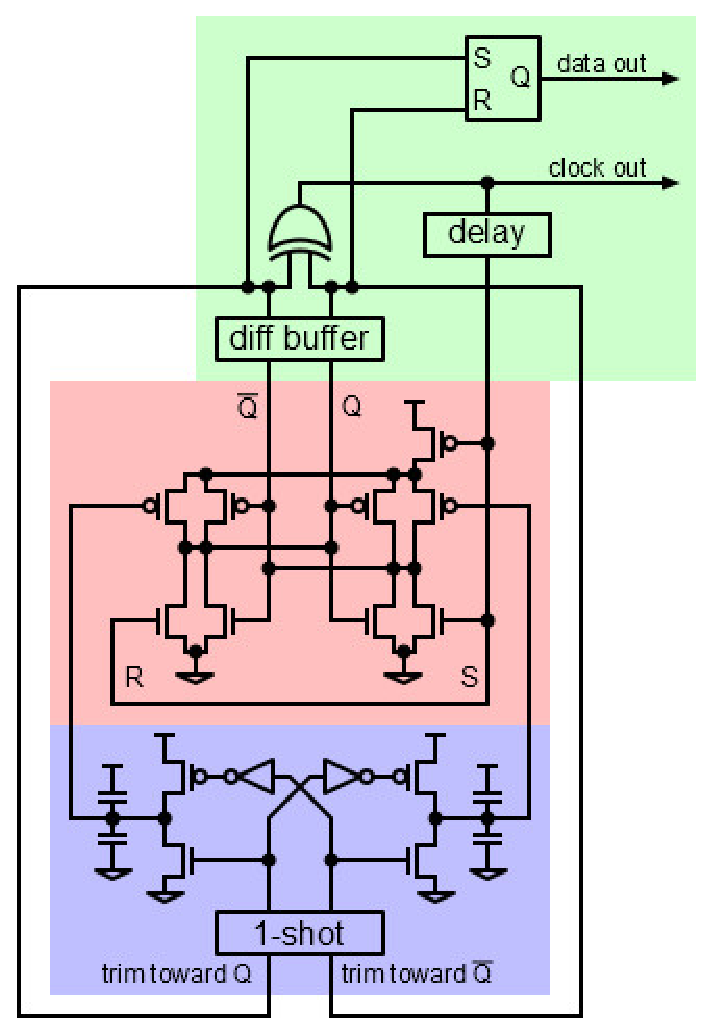
\includegraphics[width=6cm,keepaspectratio]{fig/entropy-source-circuit} % Or .pdf
%\includegraphics[width=10cm,keepaspectratio]{fig/ISK-scheme}
\caption{Circuit scheme of~the~entropy source.~\cite{UnderstandingRdRandElectronic}}
\label{fig:ES-circuit}
\end{figure}

% ....................................................
\subsection{Conditioner}
\par{
The entropy source provides random bits with some entropy, 
but due to implementation and the~feedback, it can be unbalanced 
and produce values in something close to oscillating patterns. 
For this reason, there is the~conditioner that adds them to a~256 bit pool, 
make a~set of~XOR and AES operations over lower and upper half of~the~pool 
and test health of~the~pool\footnote{The health check is done by counting six 
different bit patterns in the~256--bit pool and comparing the~counts 
with empirically chosen values. The pool is healthy only if the~numbers are 
in the~specified ranges.
}~\cite{AnalysisOfDRNG,UnderstandingRdRandElectronic}. 
If the~pool is not healthy, the~set of~operations is repeated. 
}
% ....................................................
\subsection{DRBG}\label{subsec:DRBG}
\par{
Because the~output speed of~the~conditioner is too slow (just 256 bits per few 
microseconds), 
a~deterministic random bit generator is connected to the~256 bit pool 
and every few microseconds (if the~pool is healthy) takes it as a~new seed. 
This pseudo random generator then computes 65.536 bits values using 
a 128-bit AES and put them to a~output buffer. 
From there, they can be taken by the~RdRand instruction after 64-bit 
blocks\footnote{64 bits are always taken out, no matter what size is 
the~target register of~the~instruction. Thus, it is not possible to achieve the full 
speed of the DRBG on 32-bit system, as there is no difference for the Intel 
Secure Key usage from pulling 64 bits. Just some bits are thrown away. 
See \fullref{subsec:testing:differences} for a performance test.}~\cite{AnalysisOfDRNG,UnderstandingRdRandElectronic}. 
Reseeding of~the~DRBG is required after all 1024 blocks are used, 
but usually it will reseed more frequently, 
about each 10 microseconds.~\cite[Chapter~4.4]{IntelDRNGGuide}
}
% ....................................................
\subsection{Built-in Self-Tests (BIST)}
\par{
Intel Secure Key contains also built-in self-tests. After a reset, the BIST at first test 
health of the DRBG and conditioner, then it tests the entropy source. In the first 
part, ES is disconnected, a previously determined bit sequence is 'generated' 
and the BIST checks the output with a built-in value. In second phase, 
the entropy source is connected and few sequences are generated. 
If the entropy source would be bad, the previously checked health check in conditioner would detect it. 
}

\par{
In case one of the BIST parts would not be finished correctly and the RdRand 
instruction is called, just zeros are returned and carry flag is cleared.~\cite{AnalysisOfDRNG}
}

% --------------------------------------------------------
\section{Existing Usages} 
\par{
RdRand is already used in Linux kernel for the both blocking and non-blocking pools. For the non-blocking pool({\tt /dev/urandom}), it is possible to completely feed the pool with RdRand.~\cite{KernelRdRand} For blocking pool ({\tt /dev/random}), the RdRand is used as one from more entropy sources in {\tt drivers/char/random.c}.
}

\begin{lstlisting}[frame=none, basicstyle=\footnotesize\ttfamily, language=C, numbers=none, numberstyle=\tiny\color{black},caption= {Adding RdRand (and any other platform-depending HW RNG) to blocking pool with XOR, at line 1042 in {\tt drivers/char/random.c}.~\cite{random.c}}]
for (i = 0; i < LONGS(20); i++) {
	unsigned long v;
	if (!arch_get_random_long(&v))
		break;
	hash.l[i] ^= v;
}
\end{lstlisting}

\par{
Another well-known and widely spread system already using RdRand is OpenSSL. This library added the support in version 1.0.1.~\cite{OpenSSLRandomNumbers}[Chapter 3.2 Generation] There the RdRand is provided as one engine of many and requires to be explicitly enabled.
}

\begin{lstlisting}[frame=none, basicstyle=\footnotesize\ttfamily, language=C, numbers=none, numberstyle=\tiny\color{black},caption= {Simplified example of usage of RdRand in OpenSSL~\cite{OpenSSLRandomNumbers}. }]
OPENSSL_cpuid_setup();
ENGINE_load_rdrand();
ENGINE* eng = ENGINE_by_id("rdrand");
ENGINE_init(eng);
ENGINE_set_default(eng, ENGINE_METHOD_RAND);

// Here use the engine with some RAND_ method

ENGINE_finish(eng);
ENGINE_free(eng);
ENGINE_cleanup();
\end{lstlisting}

\par{
In Windows 8, RdRand is used for example during boot for {\tt ASLR} {\em (Address Space Layout Randomization)}.~\cite{WindowsASLR,WindowsHeap}
}

% --------------------------------------------------------
\section{Security}\label{sec:security}
\par{
Security of the RNG is important, but it is hard to check. During the last few years,
 the possibility of hardware Trojans (malicious manipulation during 
 the manufacturing process) gained attention, but none was yet found. This doesn't 
necessarily means that no such exists, because detection methods are 
much more difficult than with their software kindreds, and frequently destructive. 
}

\par{
If such Trojan is not detected in software because of altering verifiable outputs 
(like AES HW Acceleration, which would not encrypt the data), 
there is not much other ways, than to slice the chip and optically inspect it. 
The verification against a "golden chip" is expensive, destructive and slow 
and requires to have the "golden", trusted chip for comparison.
Yet it can find alterations in circuits that could open some backdoors. 
But recently, another possible attack vector was described by international group
 of scientists in their work {\em Stealthy Dopant-Level Hardware Trojans}~\cite{DopantAttack} 
 in which they directly presented such attack on the Intel's RdRand.
}

\par{
The new category of attack is not modifying the circuits layout 
and is undetectable by the optical inspections, because it affects the functionality
 of transistors instead changing the layout. By slight changes 
 in doping\footnote{Doping means adding specific impurities to the clear silicon 
 to change its electric properties.}, the modified gate can become static.
}

\par{
While with a correct RdRand an attacker has a chance of $ 1/2^{128}$ to correctly guess 
a random number, the described attack could increase the chance to 
$ 1/2^n$~\cite{DopantAttack}[Chap. 3.2, page 9], but the output of such
 modified RdRand is still looking randomly. In the work is achieved  
 $n = 32$, while it still pass NIST random number test suite.
}

\par{
This kind of attack (predictability) is different from what the authors of the petition~\cite{PetitionRdRand} for removing RdRand from {\tt /dev/random} fears. Their point is that RdRand, as a part of the CPU, can actively try to reduce entropy of the pool. If it would know with what values it will be XORed (they can be in cache of the CPU), it can produce inverted value and effectively impact the pool. But I don't have enough understanding of this Linux subsystem to be able to evaluate this claim.
}
%============================================================


%=========================================================================
\chapter{The Library}\label{chap:library}
\par{
According the needs of Red Hat I created a library providing basic interface over the RdRand instruction as well as a simple application using this library. The most important reason for Red Hat's own implementation was licensing; Intel has supplied its own library providing similar interface to this one, but under its own license, which could cause problems with modification, redistribution and in combination with GNU GPL. Thus, this work has been released under GNU LGPL 2.1\footnote{For full text of the license, see \cite{GNULGPL}.}. Also, it was important to test the library and to create a documentation for it.
}

\par{
When drafting the library interface, I have at first surveyed the library example from Intel\cite{IntelDRNGGuide}, as well as OpenSSL API\cite{OpenSSLAPI}. The first draft included functions described in API in \ref{subsec:api:simple-wrappers}~(simple wrappers) and \ref{subsec:api:single-number}~(single numbers) and one function for longer sequences: \\\function{rdrand_get_bytes_retry}. 
}

\par{
Also, I planned to implement not only the usual, fast method, but also some more secure, that would avoid of relying on the security of the CSPRNG (see \fullref{sec:ISK-physical} for more details), yet I wasn't sure about an interface for this functionality.
}

\par{
This draft was discussed with Jiří Hladký. A need for more functions for longer sequences emerged from the discussion, so other functions from \ref{subsec:api:multiple}~(multiple numbers) were added and also the more secure generation was discussed. Initially, I wanted to implement the fast or more secure method switch as an state variable, set up in an initialization function or passed as an argument to the generating functions. After deeper analysis of such solution and its impact on performance and usability, I decided to implement the more secure methods as two independent functions, described in \ref{subsec:api:secure}~(secure generating).  
}

\par{
Also, the library could be used on machines with current hardware, but with legacy software where is not any support for RdRand in system libraries (for example RHEL 5). For this reason, dependency on system libraries of specific versions was declined. This means that although Linux has a {\tt X86\_FEATURE\_RDRAND} flag for testing whether the RdRand is available and function similar to wrappers in \ref{subsec:api:simple-wrappers}, it wasn't used.
}

\par{
In March 2014, this library (and the generator) was pushed into Fedora package repository~\cite{RdRandFedoraPackage,RdRandFedoraPackageBugzilla} in version 1.0.5. 
In later versions, the functionality of this library is going to be extended above the requested and described range. Specifically, some sort of encryption of generated values is going to be added to counter the possibility of predicable output.
}


\section{API} \label{sec:library-api}
\par{
The library, if installed into the system, can be included by using {\tt \#include <librdrand.h>}. In the time of this work, the library is using the following API.
}
\subsection{Constants}
\begin{description}
  \item[RDRAND\_SUCCESS] Returned by function if a random number(s) was generated correctly.
  \item[RDRAND\_FAILURE] Returned by function if a random number(s) was NOT generated correctly.
  \item[RDRAND\_SUPPORTED] Returned by \function{rdrand_testSupport} function if the CPU support RdRand.
  \item[RDRAND\_UNSUPPORTED] Returned by \function{rdrand_testSupport} function if the CPU doesn't know RdRand.
  
\end{description}


\subsection{Functions}

\subsubsection{Non-Generating Functions}

These functions are not generating any random numbers.\\

\FunctionDeclare{int}{rdrand_testSupport}{void}{Detect if the CPU support RdRand instruction. Returns {\tt RDRAND_SUPPORTED}  or {\tt RDRAND_UNSUPPORTED}.}\\

\subsubsection{Simple Wrappers}\label{subsec:api:simple-wrappers}
\par{
These methods are simply wrappers of an ASM code which generates only one n-bits number. Although these functions are provided, I expect that they will be used only infrequently. Returns {\tt RDRAND\_SUCCESS} or {\tt RDRAND\_FAILURE}.\\
}

\FunctionDeclare{int}{rdrand16_step}{uint16\_t *x}{Generates 16 bits of entropy through RdRand.}\\

\FunctionDeclare{int}{rdrand32_step}{uint32\_t *x}{Generates 32 bits of entropy through RdRand.}\\

\FunctionDeclare{int}{rdrand64_step}{uint64\_t *x}{Generates 64 bits of entropy through RdRand.}\\

\subsubsection{Generating Single Number}\label{subsec:api:single-number}
\par{
More complex functions than the previous -- in case of RdRand failure, these functions will try it again for the specified amount of times. Negative {\tt retry\_limit} implies default value with which the library is compiled. Returns {\tt RDRAND\_SUCCESS} or {\tt RDRAND\_FAILURE}.\\
}

\FunctionDeclare{int}{rdrand_get_uint16_retry}{uint16\_t *x, int retry\_limit}{Generates 16 bits of entropy through RdRand.}\\

\FunctionDeclare{int}{rdrand_get_uint32_retry}{uint32\_t *x, int retry\_limit}{Generates 32 bits of entropy through RdRand.}\\

\FunctionDeclare{int}{rdrand_get_uint64_retry}{uint64\_t *x, int retry\_limit}{Generates 64 bits of entropy through RdRand.}\\

\subsubsection{Generating Multiple Numbers}\label{subsec:api:multiple}
\par{
As a single random value is usually not enough, the library provides also functions for generating multiple bytes of random values. For higher speed, all these functions are generating values in 64bit blocks when it is possible.
These functions also accept {\tt retry\_limit} as the previous ones. Returns bytes of sucessfully generated values.\\
}

\FunctionDeclare{size\_t}{rdrand_get_bytes_retry}{void *dest, const size\_t size, int retry\_limit}{Generate {\tt size} bytes of random data.}\\


\FunctionDeclare{size\_t}{rdrand_get_uint64_array_retry}{void *dest, const unsigned int count, int retry\_limit}{Generate {\tt count} of 64bit blocks of random data.}\\

\FunctionDeclare{size\_t}{rdrand_get_uint32_array_retry}{void *dest, const unsigned int count, int retry\_limit}{Generate {\tt count} of 32bit blocks of random data.}\\

\FunctionDeclare{size\_t}{rdrand_get_uint16_array_retry}{void *dest, const unsigned int count, int retry\_limit}{Generate {\tt count} of 16bit blocks of random data.}\\

\FunctionDeclare{size\_t}{rdrand_get_uint8_array_retry}{void *dest, const unsigned int count, int retry\_limit}{Generate {\tt count} of 8bit blocks of random data.}\\

\FunctionDeclare{size\_t}{rdrand_fwrite}{FILE *f, const size\_t count, int retry\_limit}{Generate {\tt count} bytes of random values and write it to the {\tt f} stream}\\

\subsubsection{Secure Generating}\label{subsec:api:secure}
\par{
As is documented in the \fullref{chap:rdrand-instruction}, the CPU is using an~pseudorandom generator in~connection with an~entropy source. If the~user want to avoid of the~risk of taking two numbers from the same pool, that were generated from the same seed by the PRNG for some reason, it is possible to use these functions, that~guarantee\footnote{Based on description of Intel Secure Key in \fullref{subsec:DRBG}. Verification of this claim is not possible due to sealed implementation in the CPU.} by~reseeding the internal entropy pool, that each~64-bit generated value is independent on the~previous or the~next one. 
}

\par{
These methods should be used only in a single thread. 
If more threads or processes tries to generate random numbers with these two methods, 
the library has no possibility to enforce the reseeding of the PRNG and the numbers generated 
in two different threads can be from the same, non-regenerated pool.
However, between numbers in one thread, 
the reseeding is always guarranted\footnote{Accoring to known information~\cite[sec.~2.4.2]{AnalysisOfDRNG}, the DRBG requires reseeding after 512 128-bit outputs, that is 1024 of 64-bit. 
Thus if this amount of generated values is skipped, the pool has to regenerate.} 
with all reliability we can have without knowing the implementation details.
}



\FunctionDeclare{size\_t}{rdrand_get_uint64_array_reseed_delay}{uint64\_t *dest, const size\_t count, int retry\_limit}{Generate {\tt count} of 64bit values. 
Force reseed by waiting 20 microseconds before each generating. 
The delay duration was selected according a delay in Intel's reference implementation, but was doubled for sake of higher security. 
It can happen that the reseeding speed can be slower than this delay 
(if the speed with non-secure methods is markedly -- more then half -- slower 
than the ideal 800 MiB/s) and in such situation this delay may not be enough.}\\


\FunctionDeclare{size\_t}{rdrand_get_uint64_array_reseed_skip}{uint64\_t *dest, const size\_t count, int retry\_limit}{Generate {\tt count} of 64bit values. Force reseed by generating and throwing away 1024\footnote{1023 should be enough, but 1024 is better to remember.} 64-bit values per one saved. }\\


\section{RdRand Calling}
\par{
The RdRand instruction is called in three functions: \function{rdrand16_step}, \function{rdrand32_step} and \function{rdrand64_step}. In case that the compiler compiling this library knows RdRand instruction and {\tt x86intrin.h} header file is included, the three named functions are just a renaming of {\tt \_rdrandXX\_step} functions. But if the compiler do not know the instruction (for example when the version is too old), or the header file is not installed on the system, then the functions directly call a byte code.
}
\begin{lstlisting}[frame=none, basicstyle=\footnotesize\ttfamily, language=C, numbers=none, numberstyle=\tiny\color{black},caption= {Byte code called in {\tt rdrand64\_step}.}]
 asm volatile (".byte 0x48; .byte 0x0f; .byte 0xc7; .byte 0xf0; setc %1"
                      : "=a" (*x), "=qm" (err));
\end{lstlisting}

\par{
Byte code instead of instruction in the assembly language is used to support compilers who do not know about RdRand instruction. A specific example of such can be {\em RedHat Enterprise Linux 5}, whose {\tt gcc} compiler is from year 2008\footnote{According information provided by {\tt gcc} itself on any machine with RHEL 5.}. 
}

\par{
If the library is compiled for a 32-bit system, then the \function{rdrand64_step} function contain two calls of the RdRand instruction to fill lower and higher half of a 64-bit number, as it is not possible to use 64-bits registers on a 32-bit system. 
}
\section{Intelligent Generating}
\par{
Most of the functions of the library that generates an array fill the array values one by one, as it was passed to the function, just using larger data type if possible, having as little operations as possible. The \function{rdrand_get_bytes_retry} is the only one that is applying a simple heuristic for achieving the best possible speed even when passed memory area is not aligned to 64-bit blocks.
}

\par{
The function computes offset of the first 64-bit aligned block within the given memory space and then, if the offset is different than 0, it fills the few unaligned bytes at the beginning individually. After that, the generating continues like in other methods by filling 64-bit blocks until the end, potentially ending again by less than 8 bytes that needs to be filled individually (not in 64-bit chunk). Because of this approach, the function has a performance impact that can be notable on small memory areas\footnote{See \fullref{sec:testing:performance-testing} for details.}, but on large aligned areas the performance difference is almost undetectable. 
}

\section{Support Testing}
\par{
Because the RdRand instruction is not on all machines, it is necessary to provide an easy tool to check it. This is done by function \function{rdrand_testSupport}. This functions gets information about a CPU through {\tt cpuid} assembly language instruction and test a vendor string of the CPU. If the string is ``GenuineIntel'', the CPU vendor is Intel\footnote{Currently the only vendor providing this instruction. See \fullref{chap:rdrand-instruction}} and it is possible to test feature bits of the CPU for RdRand flag. Without the vendor check, it would be possible that some other vendor has another feature flag on the same bit as Intel has RdRand.
}

\section{Development and Testing Options}
\par{
Testing whether some functions that should produce random numbers are correctly working (and for example not just reusing part of memory without overwriting it) is difficult. Thus, it is possible to compile the library with defined constant {\tt STUB\_RDRAND}\footnote{When using {\tt gcc}, flag {\tt -dSTUB\_RDRAND} can be used.}. This overwrites the RdRand instruction calling, resulting in all returned bits enabled (each byte is {\tt 0xFF}). This allow to easily see, whether the generated values are correctly used in full length.
}

%============================================================


%=========================================================================

\chapter{Rdrand-Gen} \label{chap:generator}
\par{
Because the library is only for C~language, using it for example with shell scripts would be difficult. For this reason was created also a~simple executable application, which is installed with the~library, and which can be used for generating random values without the~need of using C~language by the user.
}

\par{
The generator has four optional command-line parameters to~modify its behavior. Firstly, {\tt --amount} can be used to generate specific amount of~bytes of~randomness. Suffixes K, M, G and T are accepted for easier use and when this option is not used, then the~application is generating indefinitely until it is stopped, for example by KILL signal.
}

\par{
The second parameter is {\tt --method}, which allows user to change the default method \\\function{rdrand_get_bytes_retry} for the~two reseeding functions. The~names of the~methods are made shorter for the~interaction with the~user. Third parameter {\tt --output} is used for specifying the output file -- without it, the random values are printed on {\tt stdout}. 
}

\par{
The {\tt --threads} can specify, how many threads the~generator will run in parallel for better performance. By default it is set to 2, because according to Intel~\cite{IntelArk}, in Ivy Bridge generation of CPUs (in which the~instruction was added) there are still CPUs with just two processing units (i.e. the Celeron serie).
}

\section{Underflow Recovery}
\par{
Although is stated in Intel's Software Developer Manual~\cite[chapter~7.3.17]{IntelSWManualVol1} that an exceeding of the speed of the internal generator is unlikely, and although according to {\em unverified} information (for example on StackOverflow~\cite{StackoverflowRDRANDCharacteristics}) it should not be possible in current generations (specifically on Ivy Bridge) of Intel's CPU to achieve it, we decided that the application should be working with good performance even in case of slower internal generator. The importance of this decision become even more obvious after finding that on \machine{dell-pr1700-02.lab.bos.redhat.com} the CPU wasn't able to handle more than four parallel threads reading from RdRand\footnote{Unfortunately, I cannot provide a statistic probability of such situation -- only one machine from all I have tried had this problem and I wasn't able to find that anyone other would experienced this too, which is, with regards of the currently low usage of the instruction, not surprising.}.
}

\par{
The principle is simple: By default, there is tolerance for few failures, implemented in the library itself. In such case, a new call of the RdRand instruction is made immediately after a failure. But if the RdRand is too slow, amount of the failures in a row exceeds a specific limit\footnote{Currently 3, but can be changed in the source code.}. 
}

\par{
In case of exceeding of the HW RNG speed, the generator application tries to lower the speed of acquiring. This is at first done by decrementing threads count by one and new try. If this solution is not working or is not possible (that means, when the threads count was lowered to a single thread, or was such from the beginning), delays are being inserted between calls. The delays are then lengthened with each unsuccessful call. If even in this case the HW RNG is not able to provide enough random values, the application ends with an error message\footnote{Such situation would be clearly a sign of a hardware error and thus it is questionable if the generated values would be still really random}.
}
%=========================================================================


%=========================================================================

\chapter{Testing} \label{chap:testing}
Most of the tests were done on 64-bit OS. The only exceptions are in performance section in \fullref{subsec:32vs64}.

For tests, multiple oprating systems were used.
\begin{itemize}
 \item RHEL 5, 64-bit - kernel 2.6.18-348.el5, gcc Red Hat 4.1.2-54
 \item RHEL 5, 32-bit - kernel 2.6.18-348.el5PAE, gcc Red Hat 4.1.2-54
 \item RHEL 7
 \item Fedora 19
\end{itemize}


\section{Functional Testing} \label{sec:functional-testing}
For the need of performance testing we wrote at first a testing application, as well as small set of scripts for automating of tests. And after getting the code on decent performance, we also used some statistical tests batteries, more information about them you can find in \fullref{sec:statistical-testing}. Later the rdrand-gen application was also created and tested, but it was already described in \fullref{chap:generator} as it is not a test application.

\TODO{Expand this chapter} % TODO expand this chapter


\section{Statistical Testing}\label{sec:statistical-testing}
Data

\TODO{TestU01 has some paper on their page - read it} % TODO TestU01 has some paper on their page - read it


\section{Performance Testing} \label{sec:performance-testing}
Because the performance of the RNG is important, we had to measure the performance. There are generaly two options of what performance can be measured:
\begin{itemize}
 \item Speed of the library
 \item Overal speed with writing the generated values
\end{itemize}
Althought during the development we measured both, here is tested primary the first option, just the library itself. 

The set of Bash and Python scripts in the {\tt tests/} directory is there for automatic run of the throughput test with different count of threads, parsing values and then creating graphs.

\TODO{measure also times for getting one number, one KiB... Don't forget to include any referenced test!} % TODO performance tests!

\subsection{32 and 64-bit difference}\label{subsec:32vs64}
A short comparison of performance on 32 and 64-bit system was made.
On machine \machine{hp-aladdin-01.lab.bos.redhat.com}, RHEL 5 was installed in both 32 and 64-bit version and the library was tested. As the figure~\ref{fig:32vs64} shows, the performance of 32-bit version is about half of 64-bit, which is exactly in expectations based on the~\fullref{sec:ISK-physical}.

\begin{figure}[h!]
  \centering
 \includegraphics[width=12cm]{fig/tests/32-64bit.eps} % Or .pdf
%\includegraphics[width=10cm,keepaspectratio]{fig/ISK-scheme}
\caption{The difference between 32 and 64-bit installation}
\label{fig:32vs64}
\end{figure}

\subsection{Half performance on some machines}

\subsection{Underflow}
The only machine on which I was able to achieve underflow of the HW RNG is \machine{dell-pr1700-02.lab.bos.redhat.com}.


\subsection{Specifications of referenced machines}
\TODO{More HW description} % TODO More HW description.

\machineDeclare{dell-pr1700-02.lab.bos.redhat.com}{Intel(R) Xeon(R) CPU E3-1285 v3 @ 3.60GHz}{The internal RNG is not able to handle more than four parallel threads at November 2013.}


\machineDeclare{hp-aladdin-01.lab.bos.redhat.com}{Intel(R) Core (TM) i7-3920XM CPU @ 2.90GHz}{HP elitebook 8770w, 4 GB RAM}



%=========================================================================

%=========================================================================
\chapter{Conclusion}
\par{
In this thesis I have described the~Intel Secure Key instruction RdRand and~the~library I made for its easier usage. Performed tests presented that the~real performance is not far from the~expected and~that the~produced values has a~good statistical properties and~can be considered at least as pseudorandom (\fullref{sec:testing:stat-testing}).
}

\par{
Performance testing confirmed that the~maximum speed of~RdRand is close to~the~presented value 800~MiB/s, but it also found, that a~single thread can never achieve better speed than
$800 / PUs$~MiB/s and~on IVT-EX (Intel Xeon, for example) the~production speed of~RdRand is just 400~MiB/s. Also, the~tests uncovered few performance issues on specific versions of~RHEL, namely performance drop on RHEL 6 when there is more reading threads in one application than PUs (\fullref{subsec:testing:differences}), and~a~very slow secure--generating method on RHEL 5 (\fullref{subsec:testing:fastVsSecure}).
}

\par{
The~RdRand is a~good and~fast source of~entropy. Unfortunately, revelations about NSA and~other espionage agencies throw a~shadow over this technology. One of~the~possible ways to~eliminate a~possible compromising is encrypting the~generated values by~AES in counter mode. This option is going to~be implemented in future versions of~the~library, which is already under development.
}

\par{
In current situation, there are some examples of~usage, when a~potential security risk is not harmful. The~speed allows use it for erasing hard drives with random values instead of~zeroes, when the~erasing is not slowed down by~the~RNG. Another example is ASLR or similar cases, when the~operating system has just a~little entropy collected from other sources soon after the~boot, like Windows~8 currently do~\cite{WindowsASLR}.
}

%========================================================================= 


%=========================================================================
 % viz. obsah.tex

  % Pouzita literatura
  % ----------------------------------------------
\ifczech
  \bibliographystyle{czechiso}
\else 
  \bibliographystyle{plain}
%  \bibliographystyle{alpha}
\fi
  \begin{flushleft}
  \bibliography{bibliography} 
  \end{flushleft}
  \appendix
  
  \chapter{Attachments}\label{chap:attachments}
\section{Content of the CD}
List of content on the attached CD.

\begin{description}
  \item[data -] Full results of tests used for this report.
  \item[docs -] This report and its source files (LaTeX).
  \item[literature -] Copy of used literature, if it is publicly available.
  \item[RdRand -] Clone of bgit repository with the library.
\end{description}

%\chapter{Manual}
%\chapter{Konfigra�n� soubor}
%\chapter{RelaxNG Sch�ma konfigura�n�ho soboru}
%\chapter{Plakat}



  \chapter{Glossary}\label{chap:glossary}

\begin{description}
 \item [ASLR --] Address Space Layout Randomization. Security mechanism involving randomisation of memory addresses of various system data structures to make it harder to change them in an attack.
 \item [RNG --] Random number generator.
 \item [PRNG --] Pseudorandom number generator.
 \item [CSPRNG --] Cryptographicaly secure PRNG.
 \item [TRNG --] True random number generator.
 \item [LCRNG --] Linear congruential random number generator -- a basic PRNG,
 	probably most widely used~\cite[p.~151]{CryptographyAndNetworkSecurity}.
 \item [LRNG --] Linux Random Number Generator -- a RNG used in Linux Kernel.
 \item [Entropy --] Measure of disorder and uncertainty of a system. 
 	In this report the term {\em entropy} can also refer to a random value itself 
	from an information source. See \fullref{chap:randomNumbers}.
\item [PU --] Processing Unit. A CPU with 2 cores and Hyper--Threading has 4 PUs.
\end{description}

  
\end{document}
